% !TeX encoding = UTF-8
% !TeX program = pdflatex

\documentclass[11pt]{article}
\usepackage{graphicx}
\usepackage[T1]{fontenc}
\usepackage[utf8]{inputenc}
\usepackage[italian]{babel}
\usepackage{hyperref}

\title{\textbf{easyTravel} \\ \bigskip \large Laboratorio di Architetture Software e Sicurezza Informatica \\ Ingegneria Informatica e Automatica \\ Università degli Studi di Roma "La Sapienza"}
\author{Antonini Andrea 1707560\\Cariggi Gianmarco 1698481\\Costa Marco 1691388\\Pulicati Gianluca 1708686}
\date{\today}

\begin{document}
\maketitle

\tableofcontents

\section{Introduzione}

easyTravel è un sito che permette di confrontare prezzi di voli, hotel e noleggio auto in molte
città europee, dando informazioni sul meteo della città di arrivo se la data è abbastanza vicina.

\section{Link github e tracking degli sprint}

Link github: \href{https://github.com/marcocosta96/easyTravel}{https://github.com/marcocosta96/easyTravel} \\
Link degli sprint: \href{https://docs.google.com/spreadsheets/d/14VnUUgNbMTW1_EG6KlEAEggAsf6aBKnaC1etXz5ji0I/edit#gid=12}{clicca qui} %todo

\section{User stories}

\subsection{SIGNUP, LOGIN e LOGOUT}
\begin{enumerate}
	\item As an UNREGISTERED USER I want to SING UP USING EMAIL so that I can BECOME REGISTERED USER;
	\item As an UNREGISTERED USER I want to SING UP USING GOOGLE ACCOUNT so that I can BECOME REGISTERED USER;
	\item As an UNREGISTERED USER I want to SING UP USING EMAIL AND P. IVA so that I can BECOME REGISTERED COMPANY USER;
	\item As a REGISTERED USER I want to LOGIN USING EMAIL so that I can BECOME A LOGGED USER;
	\item As a REGISTERED USER I want to LOGIN USING GOOGLE ACCOUNT so that I can BECOME A LOGGED USER;
	\item As a REGISTERED USER I want to LOGIN USING EMAIL so that I can BECOME A LOGGED COMPANY USER;
	\item As a LOGGED USER I want to LOGOUT so that I can BECOME NON-LOGGED USER;
\end{enumerate}

\subsection{Gestione Users}
\begin{enumerate}
	\item As a REGISTERED USER I want to HAVE SETTINGS so that I can CHANGE MY EMAIL;
	\item As a REGISTERED USER I want to HAVE SETTINGS so that I can CHANGE MY PASSWORD;
	\item As a REGISTERED USER I want to HAVE SETTINGS so that I can RECOVER MY PASSWORD;
	\item As a REGISTERED USER I want to HAVE SETTINGS so that I can DELETE MY ACCOUNT;
	\item As a REGISTERED USER I want to HAVE SETTINGS so that I can SET AN AVATAR;
\end{enumerate}

\subsection{Unregistered User}
\begin{enumerate}
	\item As an UNREGISTERED USER I want to RESEARCH FOR FLIGHTS so that I can COMPARE PRICES;
	\item As an UNREGISTERED USER I want to SEE THE STATISTICS so that I can SEE THE GENERAL STATISTICS;
	\item As an UNREGISTERED USER I want to SEE THE WEATHER OF THE ARRIVAL CITY so that I CAN PLAN BETTER MY TRIP;
\end{enumerate}

\subsection{Registered User}
\begin{enumerate}
	\item As a REGISTERED USER I want to CONFIRM MY EMAIL so that I can ACTIVATE MY ACCOUNT;
	\item As a REGISTERED USER I want to RESEARCH FOR FLIGHTS so that I can COMPARE PRICES;
	\item As a REGISTERED USER I want to SEE THE STATISTICS so that I can SEE THE GENERAL STATISTICS;
	\item As a REGISTERED USER I want to see the weather of the arrival city so that I can PLAN BETTER MY TRIP;
	\item As a REGISTERED USER I want to research for hotels in arrival city so that I can COMPARE PRICES;
	\item As a REGISTERED USER I want to SAVE THE SEARCH so that I can REUSE IT;
	\item As a REGISTERED USER I want to SAVE MY FAVOURITE CITIES so that I can DO RESEARCH EASILY;
	\item As a REGISTERED USER I want to DELETE FAVOURITE CITIES so that I can UPDATE MY FAVOURITE CITIES LIST;
	\item As a REGISTERED USER I want to SEE THE STATISTICS so that I can SEE GENERAL STATISTICS;
	\item As a REGISTERED USER I want to SEE THE STATISTICS so that I can SEE PERSONAL STATISTICS;
\end{enumerate}

\subsection{Company User}
\begin{enumerate}
	\item As a COMPANY USER I want to CONFIRM MY EMAIL so that I can ACTIVATE MY ACCOUNT;
	\item As a COMPANY USER I want to RESEARCH FOR FLIGHTS so that I can COMPARE PRICES;
	\item As a COMPANY USER I want to SEE THE STATISTICS so that I can SEE THE GENERAL STATISTICS;
	\item As a COMPANY USER I want to SEE THE WEATHER OF THE ARRIVAL CITY so that I can PLAN BETTER MY TRIP;
	\item As a COMPANY USER I want TO RESEARCH FOR HOTELS IN ARRIVAL CITY so that I can COMPARE PRICES;
	\item As a COMPANY USER I want to SAVE THE SEARCH so that I can REUSE IT;
	\item As a COMPANY USER I want to SAVE MY FAVOURITE CITIES so that I can DO RESEARCH EASILY;
	\item As a COMPANY USER I want to DELETE FAVOURITE CITIES so that I can UPDATE MY FAVOURITE CITIES LIST;
	\item As a COMPANY USER I want to SEE THE STATISTICS so that I can SEE GENERAL STATISTICS;
	\item As a COMPANY USER I want to RESEARCH FOR CARS so that I can RENT A CAR;
\end{enumerate}

\subsection{Admin}
\begin{enumerate}
	\item As an ADMIN I want to HAVE AN USER LIST so that I can CHECK THE USERS OF THE WEBSITE;
	\item As an ADMIN I want to HAVE SPECIAL SETTINGS so that I can DELETE USERS;
	\item As an ADMIN I want to HAVE SPECIAL SETTINGS so that I can SUSPEND THE WEBSITE;
\end{enumerate}

\section{Mockup}

\section{Schema DB}
\begin{figure}[!ht]
	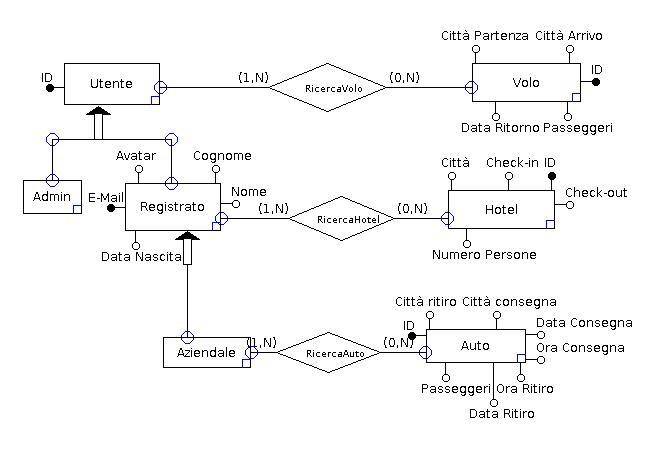
\includegraphics[width=1.2\textwidth]{progetto} % adjust width
	\caption{Schema ER}
	\label{fig:picture1}
\end{figure}

\section{Struttura controllo degli accessi}
Sono previste due modalità di accesso:
\begin{itemize}
	\item Locale: L’utente inserisce le sue informazioni direttamente sul sito.
	\item OAuth: L’utente accede tramite Google e dà il consenso al trattamento dei propri dati.
\end{itemize}

\subsection{Ruoli e diritti di accesso alle funzionalità disponibili}
I ruoli previsti all’interno dell’applicazione sono i seguenti:
\begin{itemize}
	\item Amministratore: ha accesso a tutte le impostazioni che riguardano il sito, può rimuovere commenti/utenti qualora lo ritenga necessario per evitare situazioni spiacevoli.
	\item Utente non registrato: può solamente fare ricerche di voli e consultare statistiche generali degli utenti che usano il sito.
	\item Utente registrato (Privato): oltre alle funzionalità concesse ad un utente non registrato, può fare ricerche sugli hotel, può salvare le ricerche effettuate, può impostare le città preferite e può consultare statistiche personali (come ore totali di viaggio, ecc...) e generali.
	\item Utente registrato (Aziendale): richiesta partita IVA per la registrazione, ha le stesse funzioni dell’utente privato, ma in più può fare ricerche sul noleggio auto. Può consultare solo le statistiche personali.
\end{itemize}

\section{Piano dei Test}

\end{document}
